\subsection{Radon profile classification}
\label{sec:Radon-classification}

\cite{2018MNRAS.480.2217S} identified 5 commonly recurring patterns in the stellar and gas Radon profiles of their MaNGA sample. These patterns were used to classify the Radon profiles observed in their MaNGA sample. In this work we adopt the same classification approach for the Radon profiles of the PSB galaxies and their control samples. Simplified models of 4 of the classes are shown in Figure \ref{fig:class-models}. In addition an asymmetric profile class was identified. The salient features of the Radon profile classes are listed below:

\begin{itemize}
    \item Constant, \textbf{Type-C} : Radon profile with relatively constant trace minimum angle $\hat{\theta}$ at all radii $\rho$.
    \item Inner Bend, \textbf{Type-IB} : Galaxies whose Radon profiles exhibit symmetrical variations of $\hat{\theta}$ beginning at $|\rho|=0$, then transitioning to a constant value. 
    \item Outer Bend, \textbf{Type-OB} : Galaxies with constant Radon trace angle $\hat{\theta}$  at small $|\rho|$ which transition to a different value at a greater radius. 
    \item Inner Bend + Outer Bend, \textbf{Type-IB+OB} : Galaxies with Radon profiles showing a combination of the features of Type-IB and Type OB profiles.
    \item Asymmetric, \textbf{Type-A} : The value of the $\hat{\theta}$ varies significantly with $\rho$ across opposite sides of the transform R\textsubscript{AB}. 
 \end{itemize}

\begin{figure}
    \centering
    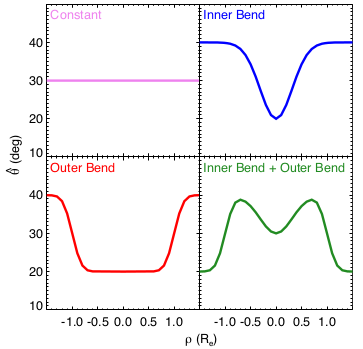
\includegraphics[width=0.8\columnwidth]{images/RadonPlots/Radon-class-models.png}
    \caption{Toy models of the Radon profile (trace angle minimum $\hat\theta$ versus radius $\rho$). The sub-plots display examples of 4 of the Radon profile classes used for classification of the RT trace plots. Upper left: Constant, Type-C; upper right: Inner Bend, Type-IB; lower left: Outer Bend, Type-OB; and lower right: Inner Bend + Outer Bend, Type-IB+OB. Source: Stark et al. (2018) figure 8.}
    \label{fig:class-models}
\end{figure}

Mathematical functions describing these Radon profile classifications have been identified by \citet[][section 3.6]{2018MNRAS.480.2217S}. This has enabled code routines to be developed which can provide automatic classification of the Radon trace profiles for galaxies in MaNGA Product Launch MPL-5. However, these automatic classification routines are not presently available in the public domain. Instead, for this work, we adopt a simple visual classification method to categorise our sample galaxy into one of the 5 Radon profile trace types listed above. The visual classification process is described in the following 3-step process:

\begin{enumerate}
    \item Firstly we obtain the MAPS datacube FITS files for the selected PSB galaxies listed in Tables \ref{tab:my-CPSBs} and \ref{tab:my-RPSBs}, and a similar number of 'normal' galaxies drawn from their respective control samples, as described in Section \ref{sec:controls}, downloaded via the MaNGA Marvin web interface.
    \item Next, we process each of datacubes through the Radon transform wrapper code to obtain PostScript output files showing the galaxy SDSS $gri$ image cutout, the MaNGA stellar velocity map, the absolute bounded Radon transform R\textsubscript{AB} plot and the Radon profile plot of $\hat{\sigma}$ versus $\rho$. An example of this output is shown in Figure \ref{fig:RT-CPSB-9493-12705-SNIP}. 
    \item  Finally we examine the output plot for each galaxy and visually assess the relative qualitative strength of each of the 5 classification features by assigning a numeric weighting as given in Table \ref{tab:features}. This method adds a semi-quantitative approach to the visual assessment process.
\end{enumerate}

\begin{table}
    \caption{Relative weighting of Radon profile feature strengths used in the  visual classification of Radon profile feature types: Constant, Inner Bend, Outer Bend, Inner Bend + Outer Bend or Asymmetric. The weighting is applied to quantify the visual appearance of the trace profile plots.}
    \label{tab:features}
    \centering
    \begin{tabular}{cl}
    \hline
    Value & Visual appearance \\
    \hline
    2 & The feature is visually predominant \\
    1 & Some evidence of the feature is apparent \\
    0 & The feature is absent \\
    \hline
    \end{tabular}

\end{table}

In order to avoid a sample induced bias the galaxies are visually assessed in alphanumerical order of their PLATEIFU file name tag. No other information is used in visual assessment process. This is intended to avoid the pitfall of assessing one group, CPSBs, RPSBs, or their respective control sample groups, where common features may be apparent in a particular group. 

After inspecting the Radon transform and associated Radon trace plots for a particular galaxy an assessment of the strength of the Radon profile type features evident in the plots. A feature strength values from Table \ref{tab:features} is assigned to each of the 5 predefined Type classes for the galaxy. Based on the relative strength values allocated a predominant feature Type (C, IB, OB, IB+OB or A) is assigned to that particular galaxy. To determine the relative predominance of Type-IB+OB features we simply sum the strength values assigned to Types IB and OB together. 
In many cases there is some uncertainty in the absolute Type assessment, i.e. only one of the 5 defines classes, a secondary assessment is made,  generally this is the primary Type plus a less evident Type, or sub-dominant Type feature. The secondary assessment may be of use later in the analysis process.

As a demonstration of the Radon profile visual classification process we select the example of the spiral galaxy 8979-12701. The Radon transform and Radon profile trace for this galaxy are shown in Figure \ref{fig:OB+IB}. Comparing the Radon trace profile with the model traces in Figure \ref{fig:class-models} and the examples given in  \citet[Figure 7 of][]{2018MNRAS.480.2217S}, the visual classification process identified the strength of the features as: C = 1, IB = 2, OB = 2, IB+OB = 2+2 = 4, and A=0. This trace profile is comparable to the Type-OB+IB model and consequently the Radon profile of this galaxy is categorised as Type-OB+IB.

The classification process outlined above was carried out independently by 3 persons in an endeavour to provide some means of eliminating personal subjectivity, in a similar manner that the Galaxy Zoo project uses large-scale public collaboration to classify galaxy morphology \citep{2017MNRAS.464.4176W}. The consensus results of the 3 independent assessments are reported in Table [TODO: of Appendix A.]

\begin{figure}
    \centering
    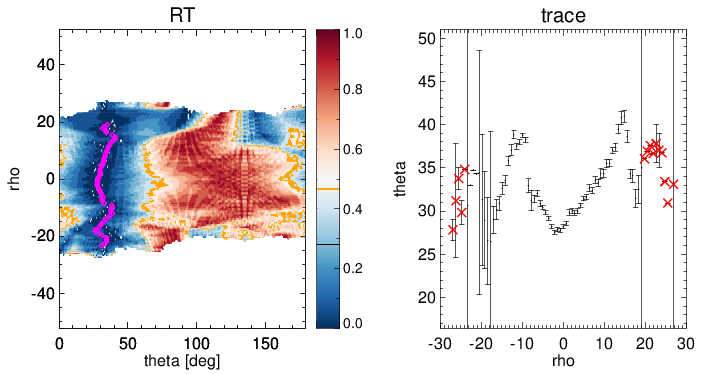
\includegraphics[width=\columnwidth]{images/RadonPlots/RT-SNIPS-NEW/8979-12701-VA-OB+IB.png}
    \caption{Example of the Radon profile visual classification method for galaxy 8979-12701. The Radon transform (RT) plot is shown in the left panel and the Radon profile trace on the right. The RT plot minimum (magenta line) shows an indication of a wide outer bend (OB) feature. The trace plot also shows a narrower inner bend (IB) feature centred at radius $\rho=0$. We therefore classify the Radon profile of this galaxy as Type-OB+IB.}
    \label{fig:OB+IB}
\end{figure}

During the classification assignment exercise  some difficulties were encountered mainly with Radon trace profiles that did not fit easily into on of the 5 classification Types. An example of this is seen in the case of 8555-3701 where a clearly defined Inner Bend appears superimposed on an asymmetric trace as shown in Figure \ref{fig:8555-3701-A+IB}. The form of this trace does not fall readily into either of the Type-A or Type-IB categories, however faces with the choice and a requirement to chose one of the 5 categories, the consensus was to classify the predominant feature as asymmetric, Type-A. The reader may disagree and opt for Type-IB, or even Type-OB+IB. This demonstrates the challenges encountered in the visual classification of Radon profiles.

\begin{figure}
    \centering
    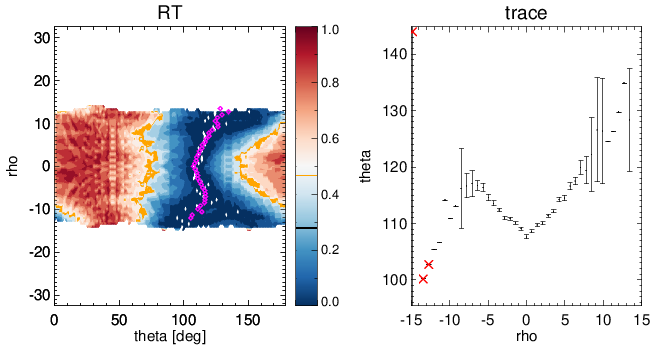
\includegraphics[width=\columnwidth]{images/RadonPlots/RT-SNIPS-NEW/8555-3701-A+IB.png}
    \caption{Radon transform and profile trace plots for the galaxy 8555-3701. An inner bend appears superimposed on a generally asymmetric trace.}
    \label{fig:8555-3701-A+IB}
\end{figure}

In many other cases bends, or velocity field disturbances, are evident as notches at well off-centre radii on otherwise constant or largely asymmetric traces. To obtain a comprehensive census at this level of detail these sub-dominant and off-centre features should be into account in a secondary analysis. Other than presenting an  assessment of these mixed secondary classifications in Table \ref{tab:full-visual-classification}, we have not pursued an analysis in this present work.




